% ============================================================
% Carbon-Aware LLM Training via Hysteresis Policy Optimization
% ICREC 2026 -- Springer LNCS
% ============================================================

\documentclass[runningheads]{llncs}

\usepackage{graphicx}
\graphicspath{{./assets/}}
\usepackage{amsmath,amssymb}
\usepackage{booktabs}
\usepackage{siunitx}
\sisetup{group-digits=false}
\usepackage{color}
\usepackage[utf8]{inputenc}

\usepackage{hyperref}
% If you use the hyperref package, please uncomment the following line
% to display URLs in blue roman font according to Springer's eBook style:
\renewcommand\UrlFont{\color{blue}\rmfamily}
\usepackage{breakurl}
\usepackage{tabularx}
\usepackage{threeparttable}

% ------------------------------------------------------------------
\begin{document}

\title{Carbon-Aware LLM Training via\\Hysteresis Policy Optimization}

\author{Simon Wittmann\orcidID{0009-0006-2291-0736} \and Julian
  Kraus\orcidID{0009-0006-1717-8376} \and Bastian
  Wiesner\orcidID{0009-0004-2594-1373} \and Saeid
  Jahandar\orcidID{0000-0002-7035-6462} \and Reinhard
German\orcidID{0000-0002-9071-4802}}

\authorrunning{S. Wittmann et al.}

\institute{
  Friedrich-Alexander University Erlangen-Nürnberg, Germany\\
  \email{\{sim.wittmann,boolean.kraus,bastian.wiesner,saeid.jahandar,
  reinhard.german\}@fau.de}
}

\maketitle

% ============================================================
% Abstract
% ============================================================
\begin{abstract}
  %The abstract should briefly summarize the contents of the paper in
  % 150--250 words.

  Large language model (LLM) training carries a critical
  environmental cost: single runs consume millions of GPU-hours and
  emit hundreds of tonnes of CO$_2$. Pausing and resuming on
  carbon-intensity thresholds is established and can cut emissions,
  but the optimal pause--resume gap (the hysteresis margin) is
  unstudied for LLM training. We present a framework that searches
  the policy space (pause threshold, resume threshold, start date)
  via adaptive grid search. Evaluating the frontier model DeepSeek~V3
  on 2025 Electricity Maps data (average, flow-traced, 5-minute, plus
  a 2022--2025 robustness check) across five grid regions, we find
  the margin is a weak lever: across 84 scenario--budget combinations
  its median optimum is 6.5~gCO$_2$eq/kWh and stays below
  20~gCO$_2$eq/kWh in 94\% of runs, while capping it at
  10~gCO$_2$eq/kWh costs a median of 0.00\,pp. Pausing is effectively
  binary, and a wide dead zone buys nothing. Sweeping checkpoint
  save/load time from 0 to 600~s over five budgets leaves the median
  optimum at 4.8~gCO$_2$eq/kWh and costs at most 0.12\,pp under the cap. In
  high-variability grids (Germany, Italy) savings reach 43.4\% and
  32.7\% at 174\% and 195\% overhead; low-variance grids (United
  States, China) yield under 10\% savings. Our results give
  region-specific design guidance for carbon-aware LLM training.

  \keywords{Carbon-aware computing \and LLM training \and Hysteresis policy \and
    Grid carbon intensity \and Temporal workload shifting \and
  Simulation \and Sustainable AI.}
\end{abstract}

% ============================================================
% 1. Introduction
% ============================================================
\section{Introduction}

The energy consumption of large language model (LLM) training has
grown dramatically. Training a single frontier model requires
millions of GPU-hours: DeepSeek~V3 (671B parameters, 14.8T tokens,
2.79M~GPU-hours)~\cite{deepseek-ai_deepseek-v3_2024}. At a per-GPU
power draw of 700~W for an NVIDIA H800 GPU during training
\cite{h800_specs} and a power usage effectiveness (PUE) of 1.27
\cite{jegham_hungry_2025}, a single run can emit hundreds of tonnes
of CO$_2$ depending on the local grid mix~\cite{patterson_carbon_nodate}.

Carbon-aware temporal workload shifting pauses training when grid
carbon intensity exceeds a threshold and resumes when it falls below
a lower one~\cite{lechowicz_pause_2023}, letting a run consume
cleaner energy without hardware modification. The threshold pair
$(\theta_p, \theta_r)$ and the start date $t_s$ jointly determine the
savings-overhead trade-off, and the gap between the two thresholds is
the hysteresis margin.

The mechanism and its analysis are well established
(Table~\ref{tab:prior}). Our policy belongs to the family of
state-dependent two-threshold pause-and-resume policies formalized by
Lechowicz~et~al.~\cite{lechowicz_pause_2023}, who charge a switching
cost per transition and derive double-threshold algorithms with
optimal competitive ratios; their threshold gap is fixed by the
switching cost rather than tuned.
Dodge~et~al.~\cite{dodge_measuring_2022} measure operational
emissions for a 6.1B-parameter model on real cloud instances and
evaluate region, time-of-day, and threshold-based pausing using
location-based marginal intensity, with a single threshold set
indirectly through a duration-increase budget. Neither calibrates how
far apart the pause and resume thresholds should be for a single,
long frontier-scale pretraining run. We study that hysteresis margin
directly, optimizing $(\theta_p,\theta_r,t_s)$ offline on historical
traces under location-based average (flow-traced) intensity, and
quantify the cost of forcing the margin wide.

\begin{table}[htb]
  \centering
  \begin{threeparttable}
    \caption{Comparison of prior workload shifting approaches. Savings
    are as reported by the respective authors.}
    \label{tab:prior}
    \small
    \begin{tabular}{@{}llc@{}}
      \toprule
      Study & Approach & Savings \\
      \midrule
      Wiesner et al.~\cite{wiesner_lets_2021}
      & Temporal shifting, generic cloud jobs
      & 3--34\% \\
      Dodge et al.~\cite{dodge_measuring_2022}
      & Flexible start, pause/resume for AI
      & up to 11.4\% \\
      Lechowicz et al.~\cite{lechowicz_pause_2023}
      & Online pause/resume, gap fixed by switch cost
      & ---\tnote{a} \\
      Hanafy et al.~\cite{hanafy_carbonscaler_2023}
      & Elastic scaling, suspend/resume baseline
      & up to 51\% \\
      Xu et al.~\cite{xu_green_2025}
      & Carbon-aware ML cluster scheduling
      & up to 41.2\% \\
      Wiesner et al.~\cite{wiesner_distributed_2026}
      & Geo-distributed, curtailment windows
      & 88--95\% \\
      Alla et al.~\cite{alla_ecoschedai_2026}
      & Predicted CI, rule-based/RL policies
      & up to 9.7\% \\
      This work
      & Static hysteresis, frontier LLMs
      & 1--43\% \\
      \bottomrule
    \end{tabular}
    \begin{tablenotes}
      \footnotesize
    \item[a] Lechowicz et al.\ report competitive-ratio improvements
      (48.2\% over carbon-agnostic), not percentage carbon savings.
    \end{tablenotes}
  \end{threeparttable}
\end{table}

Our contributions to address this gap are:
\begin{enumerate}
  \item A simulation framework for carbon-aware LLM training with
    hysteresis-based pausing, validated against a reference
    implementation and structural invariants.
  \item An adaptive grid-search optimizer that efficiently explores
    the $(\theta_p, \theta_r, t_s)$ policy space, converging within
    at most six iterations.
  \item A comprehensive empirical study of a frontier training run
    across five grid regions, establishing, to the best of our
    knowledge, the first systematic Pareto frontiers for carbon-aware
    frontier-LLM training.
  \item An empirical design rule for the hysteresis margin, based on
    84 scenario--budget combinations: optima concentrate at
    $\Delta_\theta \leq 20$~gCO$_2$eq/kWh (94\%), and enforcing
    $\Delta_\theta \leq 10$~gCO$_2$eq/kWh costs a median of 0.00\,pp
    of savings. The margin is not a sensitive tuning parameter; the
    pause threshold and the start date are. The conclusion is
    unchanged when the checkpoint cost is swept from 0 to 600\,s (40
    budget--cost combinations, at most 0.12\,pp lost by the cap).
\end{enumerate}

% ============================================================
% 2. Problem Formulation
% ============================================================
\section{Problem Formulation}

\subsection{System Model}

A single training job is defined by model parameter count $N$,
dataset token count $T$, GPU count $G$, per-GPU training power $P_t$,
per-GPU idle power $P_i$, facility PUE $\eta$, and checkpoint
save/resume durations $\tau_c, \tau_r$. It runs on a cluster in one
region whose grid carbon intensity $carbon(t)$ is a 5-minute time series.

\subsection{Hysteresis Policy}

A hysteresis policy is defined by a pause threshold $\theta_p$, a
resume threshold $\theta_r$, and a start date $t_s$. While training,
a rise of $carbon(t)$ above $\theta_p$ pauses the job, saves a
checkpoint, and idles the GPUs; while paused, a drop of $carbon(t)$
below $\theta_r$ resumes training from the last checkpoint; and $t_s$
is when training begins. The policy is feasible only if $\theta_r \leq
\theta_p$, and $\Delta_\theta = \theta_p - \theta_r$ is the
hysteresis margin. A zero margin ($\theta_r = \theta_p$) switches the
job on and off at a single threshold, whereas a positive margin opens
a dead zone in which the job keeps its current state. Prior work
fixes this gap to the switching cost~\cite{lechowicz_pause_2023} or
uses a single threshold~\cite{dodge_measuring_2022}; we treat
$\Delta_\theta$ as a free parameter to be calibrated.

\subsection{Objective}

Savings and overhead are measured against a never-pause baseline:
\begin{equation}
  S = \frac{GHG_{b} - GHG_{p}}{GHG_{b}} \times 100 \qquad
  O = \frac{T_p - T_b}{T_b} \times 100
\end{equation}
where $GHG_{b}, T_b$ and $GHG_{p}, T_p$ are the baseline and policy
emissions and times. Candidate policies are scored by
$\bigl(\alpha\,S/100 + 1 - (1-\alpha)\,O/B\bigr)/2$, with $B$ the
overhead budget. Since all experiments use $\alpha = 1$, the score
reduces to $(S/100 + 1)/2$ and the optimizer simply maximizes carbon
savings subject to $O \leq B$ (policies above $B$ are discarded,
Sect.~\ref{sec:opti-algo}); the savings-overhead balance is thus set
by $B$ alone rather than by a weighted trade-off.

% ============================================================
% 3. Simulation Framework
% ============================================================
\section{Simulation Framework} \label{sec:simulation}

\subsection{Discrete-Event Simulator}

A discrete-event simulator replays a training run under a given
policy. At each 5-minute step $\Delta t$: if training is active and
$carbon(t) > \theta_p$, the job spends $\tau_c$ saving state at full
power and then idles at $P_i$; if paused and $carbon(t) < \theta_r$,
it spends $\tau_r$ loading state (negligible for asynchronous
checkpointing) and resumes; otherwise it keeps its current state. The
energy per timestep is $E(t) = G \cdot P \cdot \eta \cdot \Delta t$
with $P = P_t$ while training and $P_i$ while paused, and emissions
are $GHG(t) = E(t) \cdot carbon(t)$. Training tokens are tracked to
completion; pause episodes extend wall-clock duration proportionally.

\subsection{Carbon Intensity Data}

\begin{table}
  \centering
  \caption{Grid carbon intensity characteristics (2025). Regions ordered
  by coefficient of variation.}
  \label{tab:grid}
  \small
  \begin{tabular}{@{}l S[table-format=3.0] S[table-format=3.2]
  S[table-format=1.2]@{}}
  \toprule
  Region & {Mean} & {Std.\ dev.} & {CV} \\
  & {(gCO$_2$eq/kWh)} & {(gCO$_2$eq/kWh)} & \\
  \midrule
  DE (Germany) & 340 & 132.37 & 0.39 \\
  SE (Sweden) & 21 & 6.42 & 0.31 \\
  IT (Italy) & 282 & 77.14 & 0.27 \\
  CN (China) & 493 & 60.85 & 0.12 \\
  US (United States) & 411 & 44.85 & 0.11 \\
  \bottomrule
\end{tabular}

\end{table}

Carbon intensity is the Electricity Maps average (consumption-based,
flow-traced) signal at 5-minute resolution for five regions in 2025,
retrieved via the historical API v3 endpoint
\path{/carbon-intensity/past-range}; the exact retrieval parameters
and the resulting series are archived in the repository. Average
intensity measures the emissions per kWh of the electricity mix
actually consumed, whereas marginal intensity measures the emissions
of the generator that would supply an additional unit of demand.
This distinction matters for load shifting: pausing computation avoids
emissions from the marginal generator, while average intensity is used
to attribute a run's footprint. Our savings are therefore attributional;
marginal-based estimates, such as those by
Dodge et al.~\cite{dodge_measuring_2022}, may yield different magnitudes
and thresholds. Table~\ref{tab:grid} summarizes the mean,
standard deviation, and coefficient of variation (CV): Germany and
Sweden have the highest CV, but Germany and Italy offer the greatest
usable arbitrage, while the low-variance United States and China
offer few clean intervals. The series is strongly autocorrelated
(lag-1 $= 0.999$, one-day lag $= 0.718$ for Germany), so
chronological trace replay is essential. Runs that would pass
31~December are replayed cyclically, repeating the same annual pattern.

% ============================================================
% 4. Optimization Method
% ============================================================
\section{Adaptive Grid-Search Optimization} \label{sec:opti-algo}

Exhaustively enumerating the 3D policy space $(\theta_p, \theta_r,
t_s)$ is computationally prohibitive: a naive grid at resolution $N$
per axis costs $O(N^2 \cdot D)$ where $D$ is the number of start-date
samples. With $N=100$ and $D=52$, brute-force requires approximately
260,000 simulations. We instead use an adaptive grid-search algorithm
inspired by trust-region optimization:
\begin{enumerate}
  \item {\bf Initialization.} A coarse grid over full bounds:
    $\theta_p \in [10, \theta_p^{\max}]$, $\theta_r \in [0,
    \theta_p^{\max}]$ with $\theta_r \leq \theta_p$, and
    $t_s$ at $D$ uniform intervals. In our experiments the maximum
    $\theta_p^{\max}$ is region-dependent: 100~gCO$_2$eq/kWh for Sweden
    and 800 for all other regions.
  \item {\bf Evaluation and selection.} Every grid point is
    simulated. Points that exceed the overhead budget $B$ are discarded.
  \item {\bf Zoom refinement.} Bounds contract around the best point
    by shrinking factor $s = 0.45$ per axis, with the grid resolution
    $N = 10$ points per axis per iteration held fixed.
  \item {\bf Iteration.} Steps 2--3 repeat for a maximum of $K = 10$ iterations.
\end{enumerate}

The initial grid always contains the extreme policy ($\theta_p =
\theta_p^{\max}, \theta_r = 0$), which does not pause under the
observed intensities, so the search is anchored by a low-overhead
candidate. The total complexity is $O(K \cdot N^2 \cdot D)$; with our
settings ($K=10, N=10, D=7$ for start-date experiments, $D=1$ for
fixed-date runs), a full optimization evaluates on the order of 3,500
candidate policies (roughly 700 for fixed-start runs), completing in
well under one minute on a single CPU core. The optimizer converges
within 5--6 iterations in all regions; later iterations improve the
score by $\leq2\times10^{-5}$.

% ============================================================
% 5. Results
% ============================================================
\section{Results}

\subsection{Experimental Setup}

DeepSeek~V3 has 671B total parameters (37B activated per token) and
14.8T training tokens, and was trained on 2048\,H800 GPUs with 2.79M
total GPU-hours~\cite{deepseek-ai_deepseek-v3_2024}. We assume a
facility PUE of 1.27~\cite{jegham_hungry_2025}.

The H800 has a TDP of 700\,W~\cite{h800_specs}. For the idle
power we adopt the measured 60\,W idle draw of the power-comparable
H100~\cite{massedcompute_h100_power,advantech_h100_h800}. We set the
checkpoint save time to 148.8\,s
(a 7B model under PyTorch distributed
checkpointing~\cite{pytorch_checkpoint}) and the resume time to 0\,s
(asynchronous checkpointing); Sect.~\ref{sec:ckpt-cost} sweeps this cost.

\subsection{Pareto Frontier Analysis}

Figure~\ref{fig:pareto} shows the combined Pareto frontiers and
Table~\ref{tab:best} the best-score configurations; for DeepSeek~V3,
single-year savings range from 43.4\% (Germany) to 6.2\% (China).
Table~\ref{tab:budgets} lists the best savings along this frontier
when the overhead budget is tightened to $B$. The budget matters in
practice: the German optimum reaches 43.4\% only by running for
2.74$\times$ the baseline duration, whereas capping overhead at 50\%
still yields 25.4\% (the 10--50\% columns are the relevant ones for
deadline-constrained jobs). In high-variability grids the frontier
reflects carbon-intensive intervals worth avoiding; Sweden plateaus
earlier because its low baseline intensity leaves fewer such windows;
the United States and China vary so little that pausing rarely finds
a cleaner interval than the one it left.

\begin{figure}[h]
  \centering
  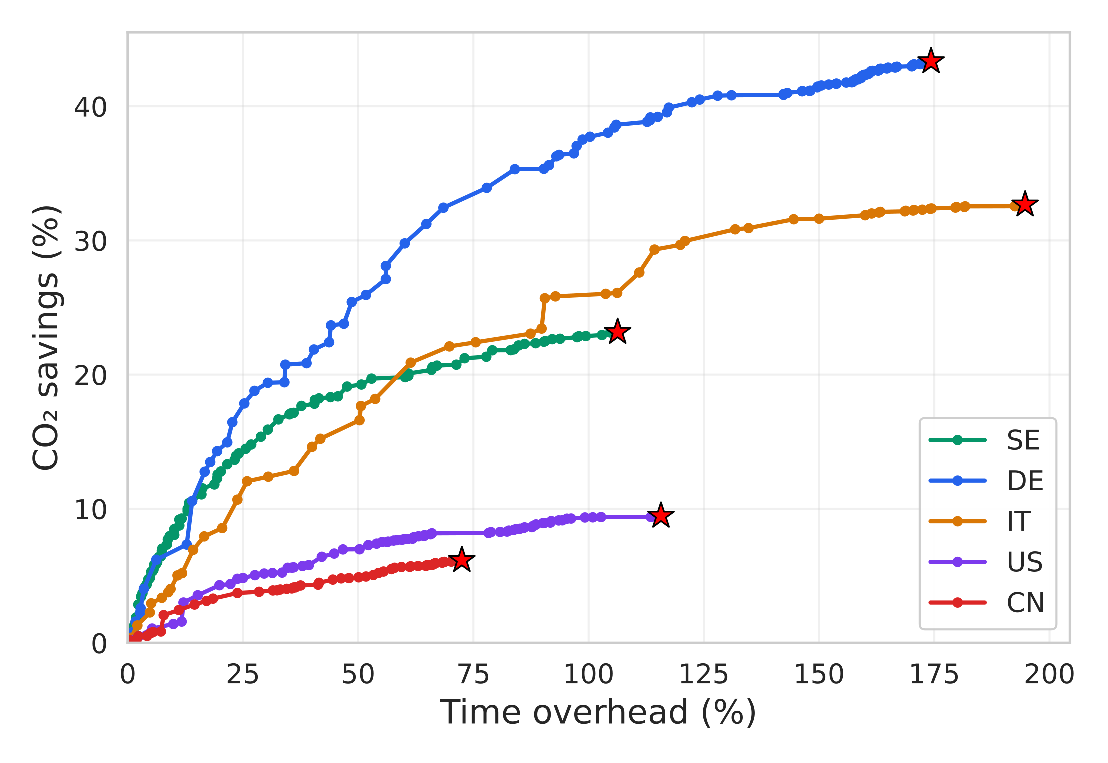
\includegraphics[width=0.64\textwidth]{savings_vs_overhead_all}
  \caption{
    Pareto frontiers for DeepSeek~V3 across five grid regions. Each
    point is a feasible policy $(\theta_p, \theta_r, t_s)$ evaluated
    on 2025 5-minute intensity data. Best-score points within 200\%
    overhead are stars.
  }
  \label{fig:pareto}
\end{figure}

\begin{table}[htbp]
  \centering
  \begin{minipage}[t]{0.46\columnwidth}\centering
    \caption{Best savings (\%) among the evaluated Pareto-optimal
      DeepSeek~V3 policies per overhead budget $B$
    (Fig.~\ref{fig:pareto}).}
    \label{tab:budgets}
    \small
    \begin{tabular}{@{}l S[table-format=2.1] S[table-format=2.1]
      S[table-format=2.1] S[table-format=2.1] S[table-format=2.1]@{}}
      \toprule
      & \multicolumn{5}{c}{Overhead budget $B$} \\
      \cmidrule(l){2-6}
      Region & {10\%} & {25\%} & {50\%} & {100\%} & {200\%} \\
      \midrule
      DE & 6.2 & 16.5 & 25.4 & 37.5 & 43.4 \\
      IT & 4.0 & 10.7 & 15.2 & 25.8 & 32.7 \\
      SE & 8.0 & 14.1 & 19.1 & 22.9 & 23.2 \\
      US & 1.4 & 4.8 & 7.0 & 9.4 & 9.5 \\
      CN & 2.1 & 3.7 & 4.8 & 6.2 & 6.2 \\
      \bottomrule
    \end{tabular}
  \end{minipage}\hfill
  \begin{minipage}[t]{0.52\columnwidth}\centering
    \caption{Best policy per region with optimized start dates; margin
      $\Delta_\theta = \theta_p - \theta_r \leq 20$~gCO$_2$eq/kWh
    everywhere.}
    \label{tab:best}
    \small
    \begin{tabular}{@{}l S[table-format=3.0] S[table-format=3.0]
      S[table-format=2.1] S[table-format=3.1]@{}}
      \toprule
      Region & {$\theta_p$} & {$\theta_r$} & {Savings (\%)} & {Overhead (\%)} \\
      \midrule
      DE & 273 & 268 & 43.4 & 174.3 \\
      IT & 247 & 230 & 32.7 & 194.7 \\
      SE &  19 &  18 & 23.2 & 106.3 \\
      US & 396 & 386 &  9.5 & 115.7 \\
      CN & 528 & 511 &  6.2 &  72.5 \\
      \bottomrule
    \end{tabular}
  \end{minipage}
\end{table}

Savings broadly track grid variability, not monotonically: Italy
beats the higher-CV Sweden, whose low absolute intensity caps the
emissions available to avoid, and the United States beats the higher-CV China.

\subsection{Threshold Space and Hysteresis Margin}

\begin{figure}
  \centering
  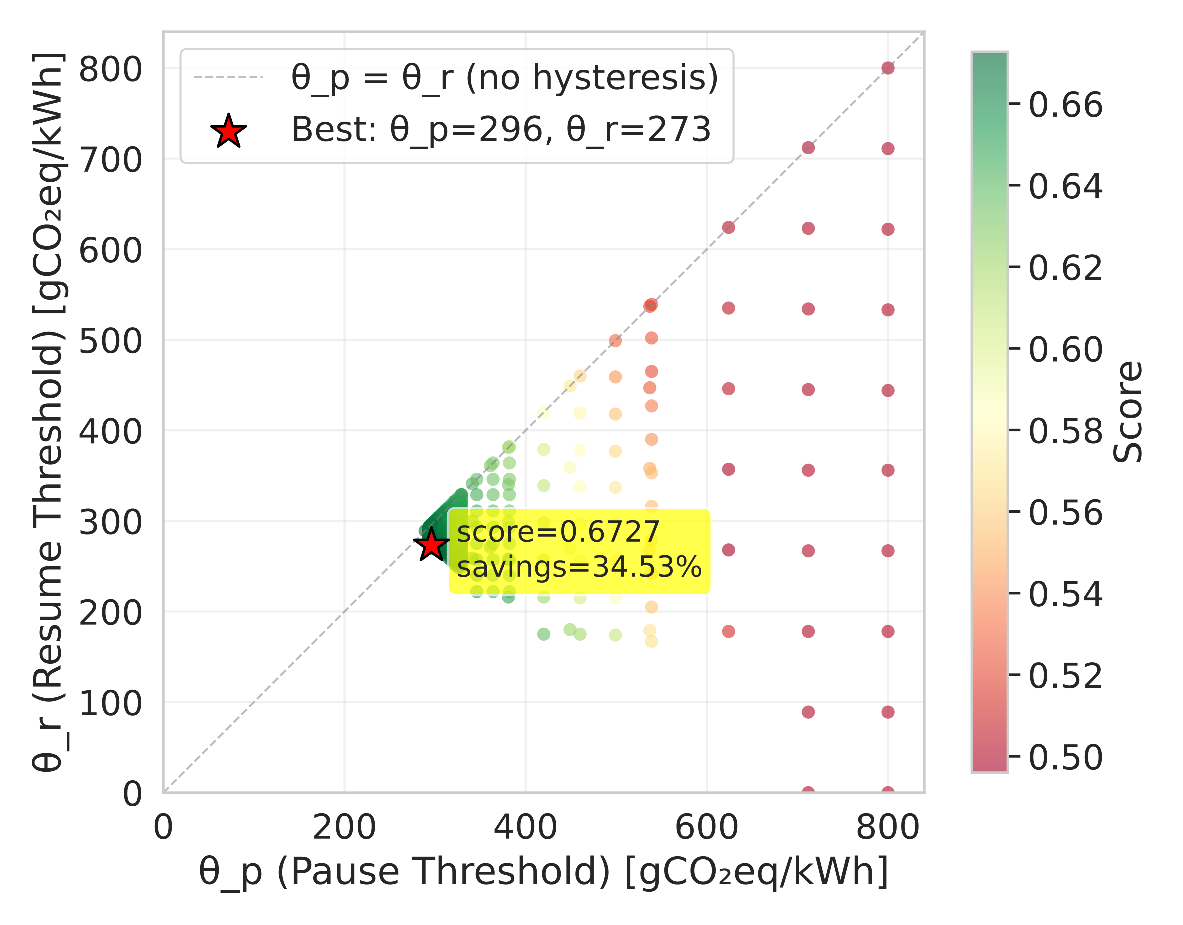
\includegraphics[width=0.52\textwidth]{threshold_space_DeepSeek_V3_DE_0101}
  \caption{
    Pause vs.\ resume threshold for DeepSeek~V3 in Germany (January 1
    start). Color encodes composite score; the diagonal
    $\theta_r=\theta_p$ marks zero-hysteresis policies.
  }
  \label{fig:threshold}
\end{figure}

The threshold analysis (Fig.~\ref{fig:threshold}) reveals that
optimal margins cluster near zero for this setup. We repeat the
optimization under five overhead budgets (10, 25, 50, 100, and 200\%)
over 19 scenarios (each region under fixed January and July starts,
  an optimizer-chosen start on 2025, and one on the 2022--2025 average;
the US July start is infeasible), yielding 84 feasible
scenario--budget pairs and 110{,}616 feasible policy evaluations
(Fig.~\ref{fig:margin}); a 2025-only subset (62 pairs) gives a median
margin of 7.0~gCO$_2$eq/kWh and $\Delta_\theta \leq 20$ in 91.9\%.

\begin{figure}[!ht]
  \centering
  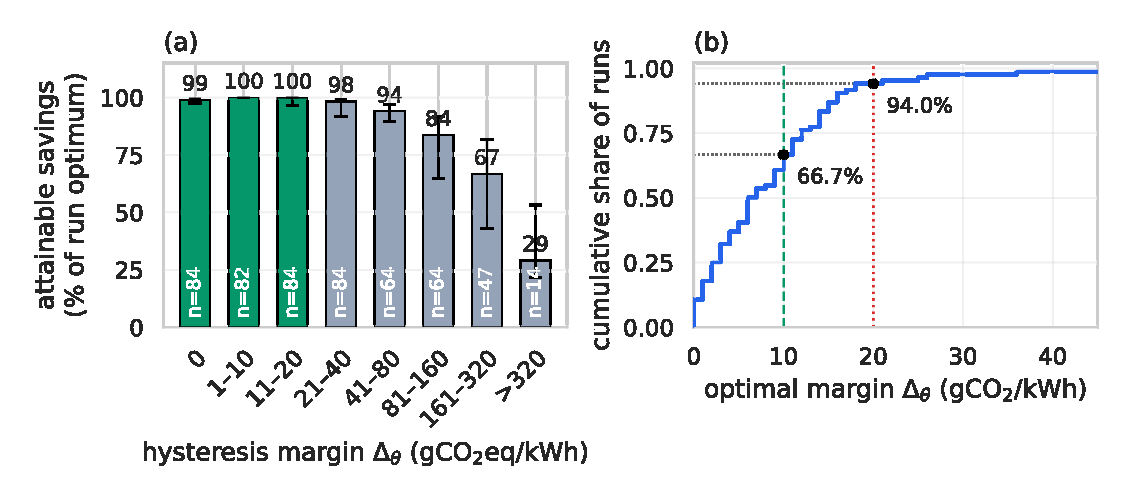
\includegraphics[width=0.795\textwidth]{margin_analysis}
  \caption{Margin analysis over 84 scenario--budget combinations.
    (a)~Best savings attainable when the margin is restricted to a bin,
    relative to the run optimum (bars: median, whiskers: interquartile
    range). (b)~Cumulative share of runs whose optimal margin falls
    below the abscissa; dashed and dotted lines mark $\Delta_\theta =
  10$ and $20$~gCO$_2$eq/kWh.}
  \label{fig:margin}
\end{figure}

The distribution of the optimal margin is strongly skewed to small
values (Fig.~\ref{fig:margin}b) with a median of 6.5~gCO$_2$eq/kWh
($\Delta_\theta \leq 10$~gCO$_2$eq/kWh in 66.7\% and $\Delta_\theta
\leq 20$~gCO$_2$eq/kWh in 94.0\% of the combinations).

Fig.~\ref{fig:margin}a prices a wide margin directly: for each bin it
shows the best savings a feasible policy in the bin can still
achieve, relative to the run optimum. Bins up to $\Delta_\theta =
20$~gCO$_2$eq/kWh stay within 1\,pp at the median; beyond that the
attainable savings fall steadily.

Capping $\Delta_\theta$ at 10~gCO$_2$eq/kWh costs a median of
0.00\,pp and a mean of 0.03\,pp of savings: 83 of 84 combinations
lose under 0.5\,pp, the worst case loses 1.05\,pp (Germany, $B =
25\%$). Capping at 20~gCO$_2$eq/kWh is cheaper still, with all 84
losing under 1\,pp. The benefit hysteresis should provide
(suppressing rapid pause/resume cycling) survives the tighter cap:
the pause count changes by a median of 0 and by $+6.7$\% on average,
and no run doubles it.

The margin is therefore an insensitive tuning parameter: once the
signal falls below the resume threshold it stays low, so waiting
longer before resuming buys little clean time while adding idle
overhead. A margin of 10~gCO$_2$eq/kWh is a safe, nearly free
default, and effort is better spent on $\theta_p$ and $t_s$.

\subsection{Sensitivity to Checkpoint Cost} \label{sec:ckpt-cost}

All preceding margin results assume a 148.8~s checkpoint cost
(measured for a 7B model). Larger checkpoints increase transition
costs and wider margins suppress pause/resume frequency. We therefore
re-run the optimization for DeepSeek~V3 in Germany (2025, optimized
start date), sweeping a symmetric save/load cost $c$ over (0, 1, 10,
30, 60, 148.8, 300, and 600~s) across the five overhead budgets. This
yields 40 combinations with 122{,}934 feasible policy evaluations.

\begin{figure}[!ht]
  \centering
  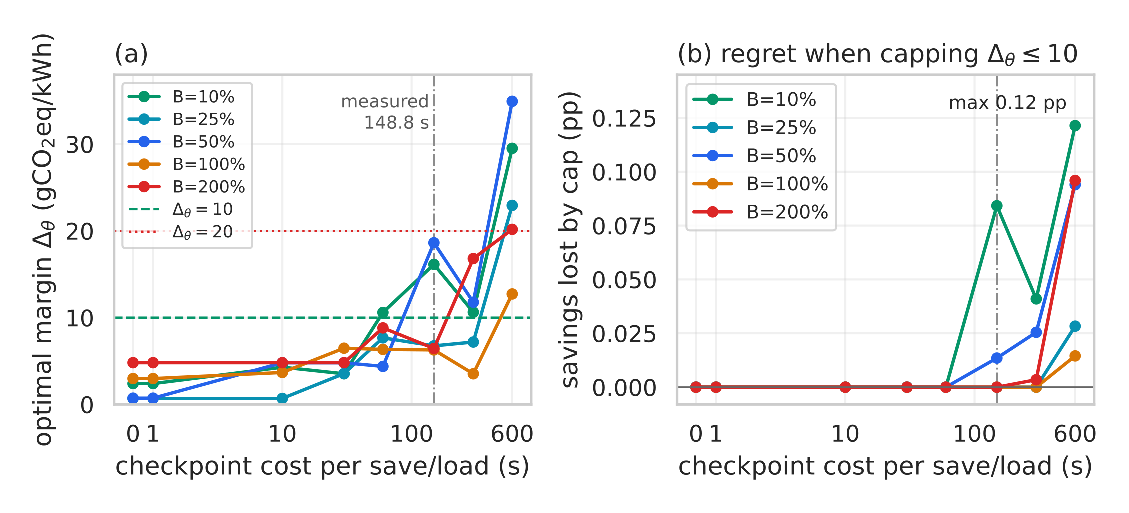
\includegraphics[width=0.83\textwidth]{checkpoint_margin}
  \caption{DeepSeek~V3 in Germany (2025) under a checkpoint-cost
    sweep: symmetric save/load cost $c$ swept over five overhead
    budgets. %(40 combinations, 122{,}934 feasible policies).
    (a)~Optimal hysteresis margin vs.\ $c$; dashed and dotted lines
    mark $\Delta_\theta = 10$ and
    20~gCO$_2$eq/kWh. (b)~Savings lost when the margin is capped at
  10~gCO$_2$eq/kWh.}
  \label{fig:ckpt-margin}
\end{figure}

As Figure~\ref{fig:ckpt-margin} shows, the optimal margin is small:
median 4.8~gCO$_2$eq/kWh, with $\Delta_\theta \leq 10$ in 72.5\% and
$\Delta_\theta \leq 20$ in 90.0\% of the 40 optima. Although higher
transition costs increase the median optimum (2.4 at $c = 0$ to
22.9~gCO$_2$eq/kWh at $c = 600$~s) and reduce pause counts (e.g., $61
\rightarrow 45$ at $B = 50\%$), no optimum exceeds 18.7~gCO$_2$eq/kWh
for $c \leq 300$~s. Capping $\Delta_\theta$ at 10~gCO$_2$eq/kWh costs
at most 0.12\,pp of savings (median 0.00\,pp; zero loss in 30 of 40
cases). Even forcing zero hysteresis costs at most 0.90\,pp.

High checkpoint costs primarily reduce achievable savings (e.g.,
losing 1.5\,pp at $B = 200\%$) rather than altering the margin.
Checkpoint cost is thus a first-order parameter for savings, but a
second-order one for hysteresis width, confirming 10~gCO$_2$eq/kWh as
a safe default even for frontier-scale models.

\subsection{Start Date Sensitivity}

Start date is a secondary lever whose value grows with the run
length. For the higher overhead budgets the optimizer consistently
selects late-winter to early-spring starts, February for Germany and
China and January for Italy and the United States, whereas at the
tightest budgets, where the run is only slightly extended, the best
start is scattered (often late summer) and contributes little.
Because a single run spans several months, beginning near the end of
the high-carbon winter aligns it with the low-carbon spring and
summer and keeps it out of the following winter peak; Germany's
cleanest months (May--June) are about half the winter level. The
effect scales with the seasonal amplitude of the grid
(Table~\ref{tab:grid}): at a 200\% budget, January versus July starts
differ by roughly 9\,pp of savings in Germany and 20\,pp in
Italy, but under 3\,pp in China. Threshold choice nonetheless dominates
the start date in every region.

% ============================================================
% 6. Discussion
% ============================================================
\section{Discussion and Conclusion}

\subsection{Limitations}
%\paragraph{Limitations}

Our simulation assumes perfect foresight, evaluating policies on
historical rather than forecasted intensity; a real deployment would
incur prediction error. The checkpoint cost is swept from 0 to 600~s
(Sect.~\ref{sec:ckpt-cost}) as a single symmetric save/load
parameter; real overhead depends on model size, sharding, and storage
bandwidth, and save/load times need not be equal. The idle power is
adopted from the power-comparable H100; the H800's idle draw under a
real training workload may differ.
The optimizer is an adaptive grid search, so ``optimum'' denotes the
best policy on a finite grid; a finer grid might shift the margins,
which is why we report the cost of a capped margin rather than
resolve the exact optimum. Finally, this work considers single-site
training; geo-distributed training could compound savings by adding
spatial flexibility.

% ============================================================
% 7. Conclusion
% ============================================================
\subsection{Conclusion}
%\paragraph{Conclusion}

We have presented a simulation framework for carbon-aware LLM
training via hysteresis-based pausing, building on the established
pause-and-resume
literature~\cite{dodge_measuring_2022,lechowicz_pause_2023}; across
five grid regions it maps the savings--overhead trade-off at frontier-LLM scale.

The central finding is that hysteresis has diminishing returns:
across 84 scenario--budget combinations the optimal margin is
6.5~gCO$_2$eq/kWh at the median and at most 20~gCO$_2$eq/kWh in 94\%
of the runs; enforcing 10~gCO$_2$eq/kWh costs a median of
0.00\,pp; sweeping checkpoint cost from 0 to 600\,s does not
change this. Wide margins waste time and checkpoint overhead
without proportional savings, whereas carbon-aware pausing can reduce
operational emissions by up to 43\% in high-variability grids at the
cost of up to 200\% time overhead.

As design guidance, high-variability grids should place $\theta_p$
near the 30--40th percentile of regional intensity (higher for very
low-intensity grids such as Sweden) and use a narrow margin of
10~gCO$_2$eq/kWh for 30--43\% savings at up to 200\% overhead;
low-variance grids yield under 10\%, where geo-distributed training
or embodied carbon trade-offs are more promising.

Future work should (1) use forecasted rather than historical
intensity for real-time deployment, (2) combine temporal shifting
with geo-distributed training, and (3) incorporate embodied carbon
to account for manufacturing emissions.

All simulation code and data, including an interactive browser-based
simulator, are available at \url{https://github.com/404Simon/TheGreenEpoch}.

% ============================================================
% References
% ============================================================
\bibliographystyle{splncs04}
\bibliography{references}

\end{document}
